\documentclass[a4j]{ujarticle}
\renewcommand{\baselinestretch}{0.85}
\usepackage[top=1.5cm, bottom=1.5cm, left=1.5cm, right=1.5cm]{geometry}
\usepackage[dvipdfmx]{graphicx, hyperref, color}
\usepackage{multirow}
\usepackage{siunitx}
\usepackage{subfig}
\usepackage{url}

\newcommand{\Tref}[1]{\mbox{表\ref{tab:#1}}}
\newcommand{\Eref}[1]{\mbox{式(\ref{eq:#1})}}
\newcommand{\Fref}[1]{\mbox{図\ref{fig:#1}}}
\newcommand{\bhline}[1]{\noalign{\hrule height #1}}

\hypersetup{
	setpagesize=false,
	bookmarksnumbered=true,
	bookmarksopen=true,
	colorlinks=true,
	linkcolor=black,
	citecolor=black
}

\begin{document}

	\begin{flushright}
		MDLab GM資料\\
		21年10月12日(火)
	\end{flushright}

	\begin{center}
		{\Large	腹部超音波画像からの腫瘍検出}
	\end{center}

	\begin{flushright}
		{\large B3  原 英吾}\\
	\end{flushright}

	\section{研究背景および目的}
        \begin{figure}[h]
            \begin{minipage}{.59\textwidth}
                \begin{itemize}
                    \item 背景
                    \begin{itemize}
                        \item 検査実施者は超音波器具の操作と同時に診断を行わなければならず高難易度
                        \item 肝臓は沈黙の臓器と呼ばれ,炎症やガンがあっても初期には自覚症状がほとんどない
                        \begin{itemize}
                            \item 自覚しているときには重症化しているケースが多い
                        \end{itemize}
                        \item 機械学習による診断のサポート
                        \begin{itemize}
                            \item 提供されているデータセットには,\Fref{ex}の様に明らかなアノテーション不足のある画像が存在する
                        \end{itemize}
                    \end{itemize}
                    \item 目的
                    \begin{itemize}
                        \item 既存の研究を踏まえたモデルの精度向上
                        \begin{itemize}
                            \item noisy label\footnotemark[1]による精度低下の改善
                        \end{itemize}
                        \item 超音波支援システムの開発
                        \begin{itemize}
                            \item 早期発見につながると良い
                        \end{itemize}
                    \end{itemize}
                \end{itemize}
            \end{minipage}
            \begin{minipage}{.39\textwidth}
                \centering
				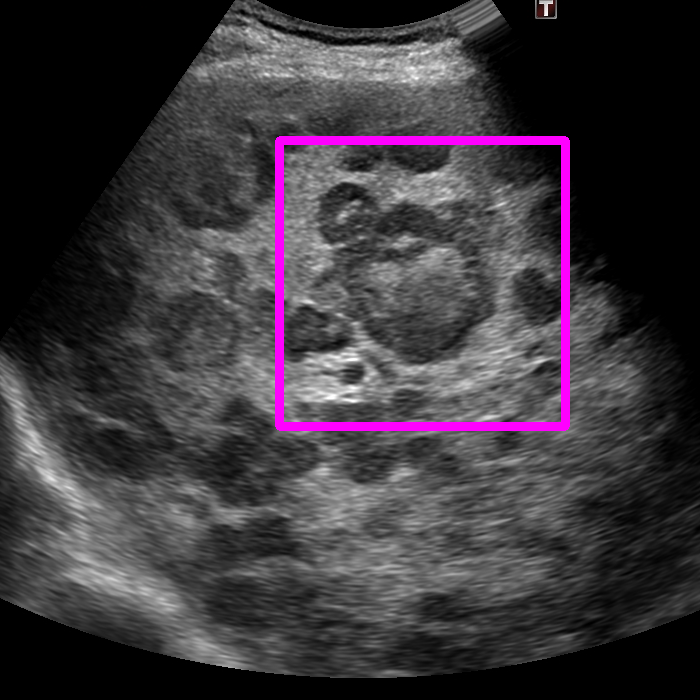
\includegraphics[width=.9\linewidth]{../fig/pseudo.png}
				\caption{アノテーション不足のある診断画像例}
				\label{fig:ex}
            \end{minipage}
        \end{figure}
        \footnotetext[1]{今回は\Fref{ex}の様なアノテーションが不足しているものを指す}
        \addtocounter{footnote}{1}

	\section{これまでの研究のまとめ}
        \begin{itemize}
            \item データセット
            \begin{itemize}
                \item 国立研究開発法人日本医療研究開発機構(AMED)\footnote{\url{https://www.amed.go.jp/}}が提供している約9万人に及ぶ以下のデータが付随している
                \begin{itemize}
                    \item 腹部超音波画像,ROI
                    \item 年齢,性別
                \end{itemize}
            \end{itemize}
            \begin{figure}[h]
                \centering
                \subfloat[性別毎の画像枚数]{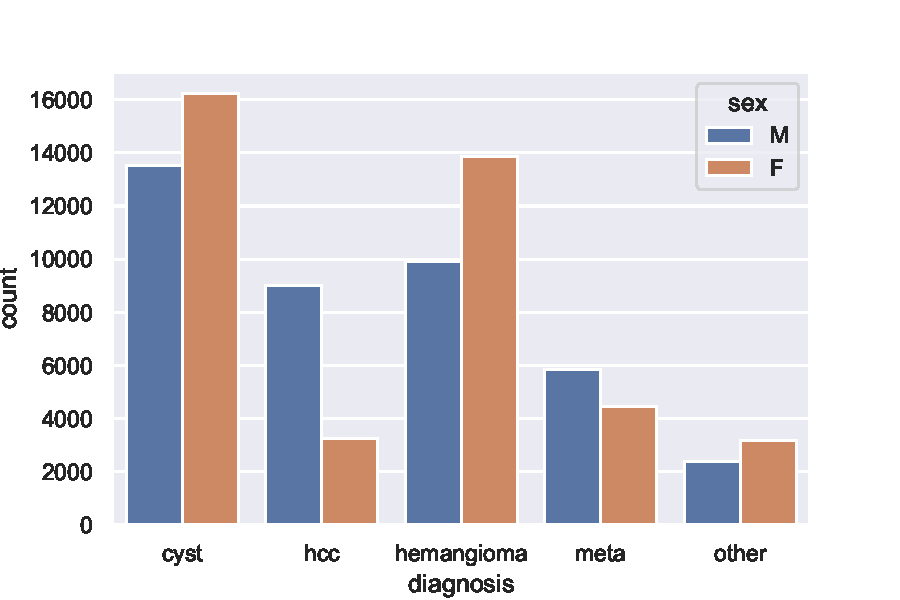
\includegraphics[width=.49\linewidth]{../fig/sex.pdf} \label{fig:sex}}
                \subfloat[診断名毎の年齢分布]{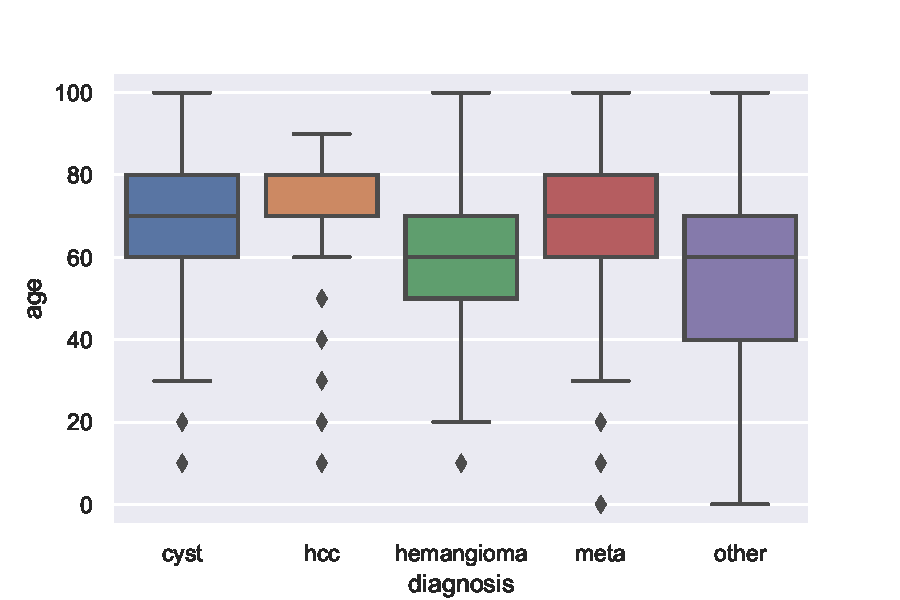
\includegraphics[width=.49\linewidth]{../fig/age.pdf} \label{fig:age}}
                \caption{データセットに含まれているメタデータの分布}
            \end{figure}
            \begin{itemize}
                \item 性別(\Fref{sex})
                \begin{itemize}
                    \item 肝細胞癌(hcc)は男性が罹患しやすい
                    \item 血管腫(hemangioma)は女性が罹患しやすい
                \end{itemize}
                \item 年齢(\Fref{age})
                \begin{itemize}
                    \item 肝細胞癌(hcc)は比較的高齢者が罹患しやすい
                    \item 単純嚢胞(cyst),血管腫(hemangioma),転移性癌(meta)の分布にははあまり特徴がない
                    \item その他(other)は分布が広がっている
                    \begin{itemize}
                        \item 様々な診断が含まれているため
                    \end{itemize}
                \end{itemize}
            \end{itemize}
        \end{itemize}

    \section{前回のLTからの進捗}
        \begin{itemize}
            \item データセットの画像サイズとそれに対するbboxの割合を算出
            \begin{figure}[h]
                \centering
                \subfloat[診断名毎の画像サイズ$(h \times w)$の分布]{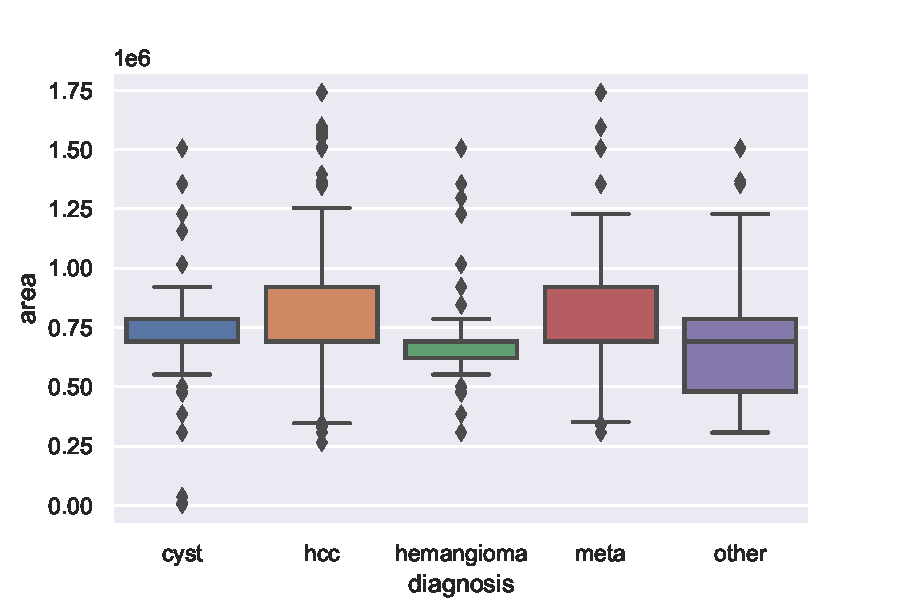
\includegraphics[width=.49\linewidth]{../fig/area.pdf} \label{fig:area}}
                \subfloat[診断名毎のbboxの割合]{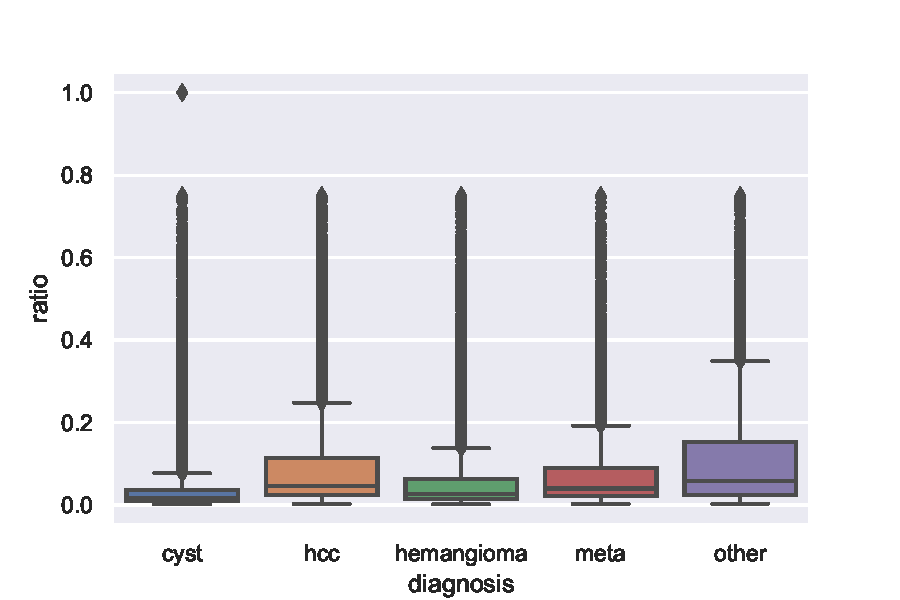
\includegraphics[width=.49\linewidth]{../fig/ratio_bbox.pdf} \label{fig:ratio_bbox}}
                \caption{データセットに含まれている画像やbboxのサイズ}
            \end{figure}
            \begin{itemize}
                \item 画像サイズの分布(\Fref{area})
                \begin{itemize}
                    \item 先輩方の先行研究で排除されていた$400 \times 400$以下の画像がcyst(単純嚢胞)に3枚含まれている
                    \item hemangioma(血管腫)は比較的画像サイズが統一されている
                    \begin{itemize}
                        \item 血管腫であるから腫瘍の大きさにあまり偏りが生じていない?
                    \end{itemize}
                \end{itemize}
                \item 診断名毎のbboxの割合(\Fref{ratio_bbox})
                \begin{itemize}
                    \item cyst(単純嚢胞)は他の診断と比べてbboxの割合が低い($\displaystyle \frac{1}{2}$程度)
                    \item cyst(単純嚢胞)での1に近い画像群は先($400 \times 400$以下)の画像と同じ
                    \begin{itemize}
                        \item 腫瘍全体が映し出されている画像
                    \end{itemize}
                \end{itemize}
            \end{itemize}
            \item 他のモデルを使う環境を整えた
            \begin{itemize}
                \item YOLOXの動作確認
                \begin{itemize}
                    \item 超音波画像での学習は行っていない
                \end{itemize}
                \item HRNet\footnote{\url{https://github.com/HRNet}}の動作確認
                \begin{itemize}
                    \item 超音波画像での学習は行っていない
                    \item 論文の閲読
                    \begin{itemize}
                        \item Deep High-Resolution Representation Learning for Human Pose Estimation \cite{hrnet}
                        \item Deep High-Resolution Representation Learning for Visual Recognition \cite{recognition}
                        \item HigherHRNet: Scale-Aware Representation Learning for Bottom-Up Human Pose Estimation \cite{bottom}
                    \end{itemize}
                \end{itemize}
            \end{itemize}
            \item GPGPUでの環境を構築
        \end{itemize}
    
    \section{今後の課題\&スケジュール}
		\begin{itemize}
			\item 10/26まで
			\begin{itemize}
                \item データが扱いにくいので整理する
                \item その形式のDataLoaderを作成
                \begin{itemize}
                    \item ImageFolderを継承したらできそう?
                    \item COCO Datasetの様にjson形式で保存すると便利かも?
                \end{itemize}
            \end{itemize}
			\item できるだけ早めに
			\begin{itemize}
                \item 研究の方向性を決める
                \item 他のモデルで実験を行ってみる
                \begin{itemize}
                    \item YOLOX
                    \item HRNet
                \end{itemize}
                \item Confident Learning \cite{cleanlab} を利用してみる
                \begin{itemize}
                    \item ラベルにノイズが含まれていると予想されるデータセットに対して精度を向上させることのできる学習を行う手法
                    \item pipでインストールできるcleanlab\footnote{\url{https://github.com/cleanlab/cleanlab}}というライブラリを用いることで簡単に使える
                    \begin{itemize}
                        \item 調べてみたら元はKeras?
                    \end{itemize}
                \end{itemize}
            \end{itemize}
		\end{itemize}

    \begin{thebibliography}{9} 
        \bibitem{hrnet} Ke Sun, Bin Xiao, Dong Liu, and Jingdong Wang. \href{https://arxiv.org/pdf/1902.09212.pdf}{Deep High-Resolution Representation Learning for Human Pose Estimation}, 2019.
        \bibitem{recognition} Jingdong Wang, Ke Sun, Tianheng Cheng, Borui Jiang, Chaorui Deng, Yang Zhao, Dong Liu, Yadong Mu, Mingkui Tan, Xinggang Wang, Wenyu Liu, and Bin Xiao. \href{https://arxiv.org/pdf/1908.07919.pdf}{Deep High-Resolution Representation Learning for Visual Recognition}, 2020.
        \bibitem{bottom} Bowen Cheng1, Bin Xiao2, Jingdong Wang2, Honghui Shi1,3, Thomas S. Huang1, and Lei Zhang. \href{https://arxiv.org/pdf/1908.10357.pdf}{HigherHRNet: Scale-Aware Representation Learning for Bottom-Up Human Pose Estimation}, 2020.
        \bibitem{cleanlab} Curtis G. Northcutt, Lu Jiang, and Isaac L. Chuang. \href{https://arxiv.org/pdf/1911.00068.pdf}{Confident Learning: Estimating Uncertainty in Dataset Labels}, 2021.
    \end{thebibliography}
\end{document}
